\section{POI空间分析}

\subsection{POI获取}

\begin{frame}[c]{微博数据接口}
    新浪微博提供了API方便第三方程序访问微博丰富的数据资源

    \begin{figure}
        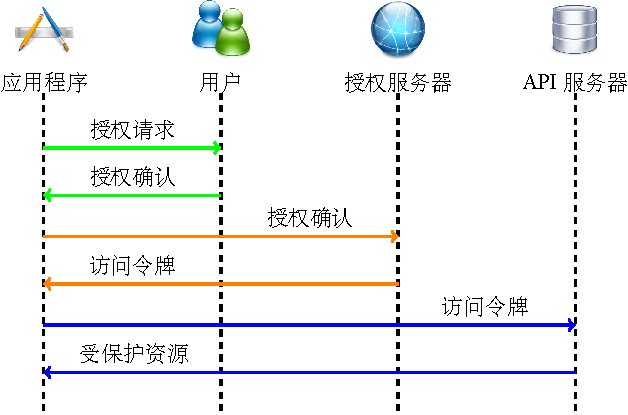
\includegraphics[scale=0.8]{figures/api.pdf}
    \end{figure}

    \pause
    \alert{HTTP Get}
\end{frame}

% \begin{frame}[t]{微博数据接口}
    

%     \vspace{0.5em}
%     \pause
%     \begin{itemize}
%     \item location/geo/address\_to\_geo $\rightarrow$  根据地址返回地理信息坐标 
%     \item location/pois/show\_batch $\rightarrow$ 批量获取POI点的信息
%     \item location/citycode $\rightarrow$ 城市代码对应表
%     \item place/nearby/pois $\rightarrow$ 获取附近的POI点
%     \end{itemize}
% \end{frame}

\begin{frame}[c]{POI空间分析(获取)}
    POI是新浪微博用户在使用过程中自行添加附近的热门位置

    \vspace{1em}
    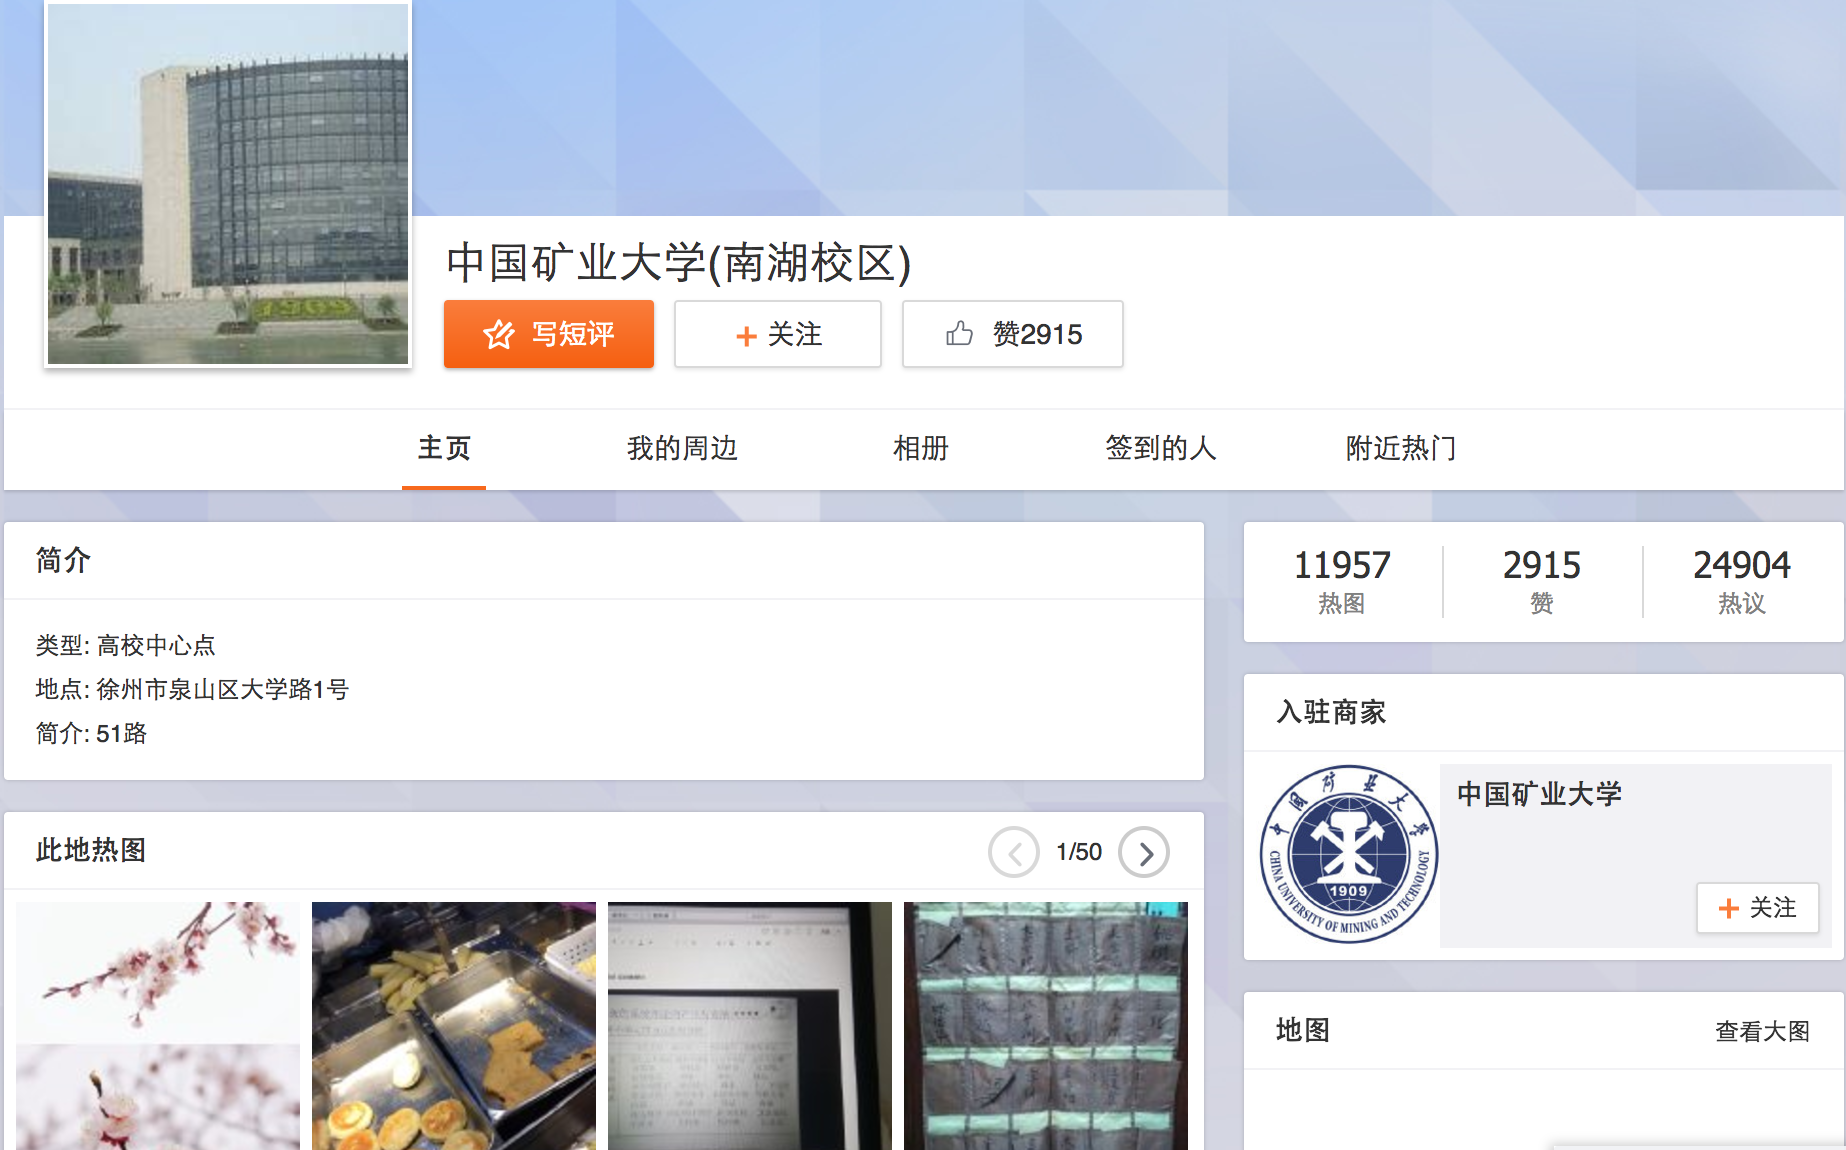
\includegraphics[scale=0.3]{figures/webpoi.png}
\end{frame}

\begin{frame}[c]{POI空间分析(获取)}
    \begin{columns}
        \begin{column}{0.5 \textwidth}
            \alert{place/nearby/pois}
            \vspace{1em}
            \begin{itemize}
                \item \textbf{Lat:} 纬度
                \item \textbf{Long:} 经度
                \item \textbf{Range:} 查询半径
            \end{itemize}
        \end{column}
        
        \pause
        \begin{column}{0.5 \textwidth}
            \begin{itemize}
                \item \alert{投影}

                Lambert 投影

                \pause
                \item \alert{栅格化}

                \vspace{0.5em}
                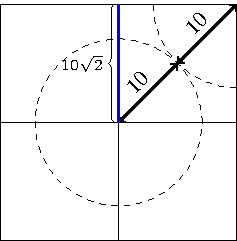
\includegraphics[scale=0.8]{figures/query.pdf}

                \pause
                \item \alert{坐标反算}

                适应API接口

            \end{itemize}
            
        \end{column}
    \end{columns}
\end{frame}

\subsection{统计分析}

\begin{frame}[c]{POI空间分析(统计)}
    \begin{columns}
        \vspace{0.5em}
        \begin{column}{0.5 \textwidth}
            \alert{热门签到地点}: sortBy, take

            \pause
            \begin{enumerate}
                \item 星光公益站
                \item 浦东机场
                \item 厦门高崎国际机场
                \item 中关村
                \item 深圳宝安机场
                \item 丽江古城
                \item 成都双流国际机场
                \item 望京
                \item 首都机场T3航站楼
                \item 广州白云机场
            \end{enumerate}
        \end{column}

        \pause
        \vspace{0.5em}
        \begin{column}{0.5 \textwidth}
            \alert{热门签到类别}: groupBy, reduce

            \pause
            \vspace{2em}
            
\includegraphics[scale=0.4]{figures/poi_category.png}
        \end{column}
    \end{columns}
\end{frame}



\subsection{同位模式}

\begin{frame}[c]{POI空间分析(同位模式)}
    \alert{关联规则算法}

    \vspace{1em}
    \begin{itemize}
        \item 事务项$T$,由集合$I_1,I_2,\ldots,I_m$组成
        \item $P \in T, Q \in T$,规则$P \rightarrow Q$
        \item 置信度约束 $c(P \rightarrow Q) \ge min\_c$
        \item 支持度约束 $s(P \rightarrow Q) \ge min\_s$
    \end{itemize}

    \pause
    \vspace{1em}
    \alert{Apriori算法}

    \begin{itemize}
        \item 频繁项的子 集必须也是频繁的
        \item 非频繁项的超集必定非频繁
    \end{itemize}
\end{frame}

\begin{frame}[t]{POI空间分析(同位模式)}

    \begin{alert}{单主题空间关联规则}
     \begin{equation}
        P_1\wedge P_2\wedge \ldots \wedge P_m \rightarrow Q_1\wedge Q_2\wedge \ldots \wedge Q_n(s\%, c\%)
    \end{equation}
    \end{alert}
    % % 单主题空间关联规则
    
    \pause
    \begin{alert}{多主题同位模式}
            \begin{equation}
                R(a_1,b_1) \Leftrightarrow (distance(a_1,b_1)\le d)
            \end{equation}

            \pause
            \begin{figure}
                \centering
                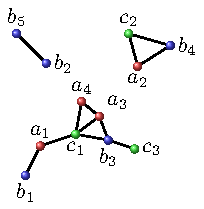
\includegraphics[scale=1.0]{figures/spatialrelation.pdf}
            \end{figure}
    \end{alert}

    % 其中$P_i$和$Q_j$中至少有一个为空间谓词
\end{frame}

% \begin{frame}[c]{POI空间分析(同位模式)}
%     多主题同位模式
%     \begin{equation}
%         R(a_1,b_1) \Leftrightarrow (distance(a_1,b_1)\le d)
%     \end{equation}

%     \pause
%     \begin{figure}
%         \centering
%         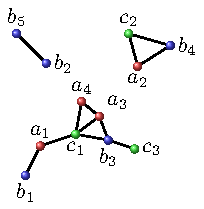
\includegraphics[scale=1.0]{figures/spatialrelation.pdf}
%     \end{figure}
% \end{frame}

\begin{frame}[c]{POI空间分析(同位模式)}
    \begin{columns}
        \begin{column}{0.3 \textwidth}
            \begin{figure}
                \centering
                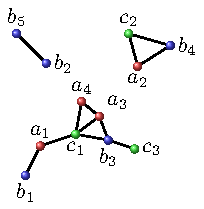
\includegraphics[scale=0.8]{figures/spatialrelation.pdf}
            \end{figure}
        \end{column}

        \begin{column}{0.7 \textwidth}
            \alert{参与率}
            \begin{equation}
                PR(c,f_i)=\frac{|\pi_{f_i}(table\_instance(c))|}{|table\_instance(\{f_i\})|}
            \end{equation}
            $PR(\{A,B,C\},A)=2/4=0.5$
            
            $PR(\{A,B,C\},B)=2/5=0.4$
            
            $PR(\{A,B,C\},C)=2/3=0.67$

            \pause
            \vspace{0.5em}
            \alert{参与度}
            \begin{equation}
                PI(c)=min_{i=1}^{k}\{PR(c,f_i)\}
            \end{equation}

            $PI(\{A,B,C\})=min(0.5,0.4,0.67)=0.4$
        \end{column}
    \end{columns}
\end{frame}

\begin{frame}[t]{POI空间分析(同位模式)}
    Spatial-Spark二阶模式生成

    \vspace{1em}
    \begin{figure}
        \centering
        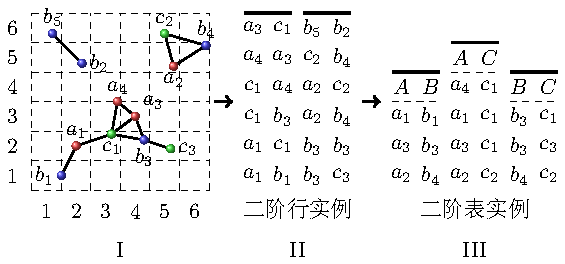
\includegraphics[scale=0.6]{figures/two_order.pdf}
    \end{figure}
    

    \pause
    键值相等判断
    \begin{figure}
        \centering
        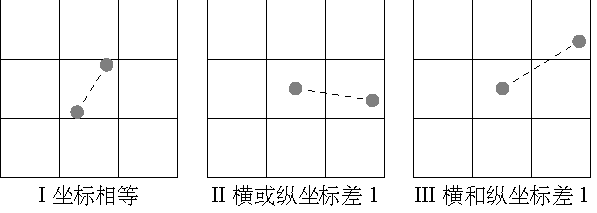
\includegraphics[scale=0.5]{figures/keyequal.pdf}
    \end{figure}
  
\end{frame}

\begin{frame}[t]{POI空间分析(同位模式)}

% \begin{algorithm}[H]
% \begin{algorithmic}[1]
% \FOR{$i=1$ to $N$}
% \FOR{$j=1$ to $JJJJ$}
% \STATE $energy[i*JJJ+j] =$ 
% $ interpolate(AAA[i*JJJ+j], ZZZ)$
% \ENDFOR
% \ENDFOR
% \end{algorithmic}
% \caption{pseudocode for the calculation of }
% \label{alg:seq}
% \end{algorithm}
\begin{algorithm}[H]
\tiny
\caption{co-location算法}
\begin{algorithmic}[1]   
\REQUIRE  ~~\\  
点集:points;\\  
距离阈值:d;\\
参与度阈值:threshold;\\  
\ENSURE ~~\\  
空间同位模式:colocation patterns; \\
\STATE $P_2$ = Spatial-Spark.join(points, d, threshold)
\WHILE{$P_k$ is not empty and $k$ < N} 
\pause
\STATE // \alert{Join操作,RowPattern重写}
\STATE $C_{k+1}$ = gen\_candinate\_cocolation($P_k$,$k$) $//$k+1阶候选集合
\pause
\STATE // \alert{距离阈值比较}
\STATE $C_{k+1}$ = pruning($C_{k+1}$, $d$)
\pause
\STATE // \alert{reduce生成表实例}
\STATE $T_{k+1}$ = gen\_table\_ins()$//$生成表实例
\pause
\STATE // \alert{threshold 筛选}
\STATE $P_{k+1}$ = Select\_Colocation\_Pattern($T_{k+1}$, threshold) $//$ 筛选表实例
\pause
\STATE $k$ = $k+1$ $//$下一轮迭代
\pause
\ENDWHILE 
\pause
\RETURN $P_2$,$\dots$,$P_k$
\end{algorithmic}
\end{algorithm} 
\end{frame}


\begin{frame}[c]{POI空间分析(同位模式)}
    \scriptsize
    \begin{columns}
        \begin{column}{0.333 \textwidth}
        \alert{上海市}

        \vspace{1em}
        (高等院校,校园生活):0.556

        \vspace{1em}
        (高等院校,日本料理):0.472

        \vspace{1em}
        (高等院校,西餐厅):0.454
        \vspace{1em}

        (高等院校,甜品店):0.451
        \vspace{1em}

        (高等院校,培训机构):0.446
        \vspace{1em}

        (高等院校,医院):0.443
        \vspace{1em}

        (高等院校,糕饼店):0.441
        \vspace{1em}

        (高等院校,餐饮美食):0.432
        \end{column}

        \begin{column}{0.333 \textwidth}
        \alert{武汉市}
        \vspace{1em}

        (高等院校,校园生活):0.531
        \vspace{1em}

        (高等院校,图书馆):0.528
        \vspace{1em}

        (高等院校,糕饼店):0.384
        \vspace{1em}

        (高等院校,快餐厅):0.368
        \vspace{1em}

        (高等院校,四川菜):0.361
        \vspace{1em}

        (高等院校,火锅店):0.358 
        \vspace{1em}

        (高等院校,连锁酒店):0.354
        \vspace{1em}

        (高等院校,医院):0.328
        \end{column}

        \begin{column}{0.333 \textwidth}
        \alert{重庆市}

        \vspace{1em}
        (高等院校,校园生活):0.306
        \vspace{1em}

        (高等院校,ATM):0.238
        \vspace{1em}

        (高等院校,科研机构):0.224
        \vspace{1em}

        (高等院校,图书馆):0.224
        \vspace{1em}

        (高等院校,超市):0.217
        \vspace{1em}

        (高等院校,特色餐厅):0.215
        \vspace{1em}

        (高等院校,电子卖场):0.210
        \vspace{1em}

        (高等院校,KTV):0.205
        \end{column}
        
    \end{columns}
\end{frame}

\begin{frame}[c]{POI空间分析(同位模式)}
    \alert{(高等院校, 培训机构)}

    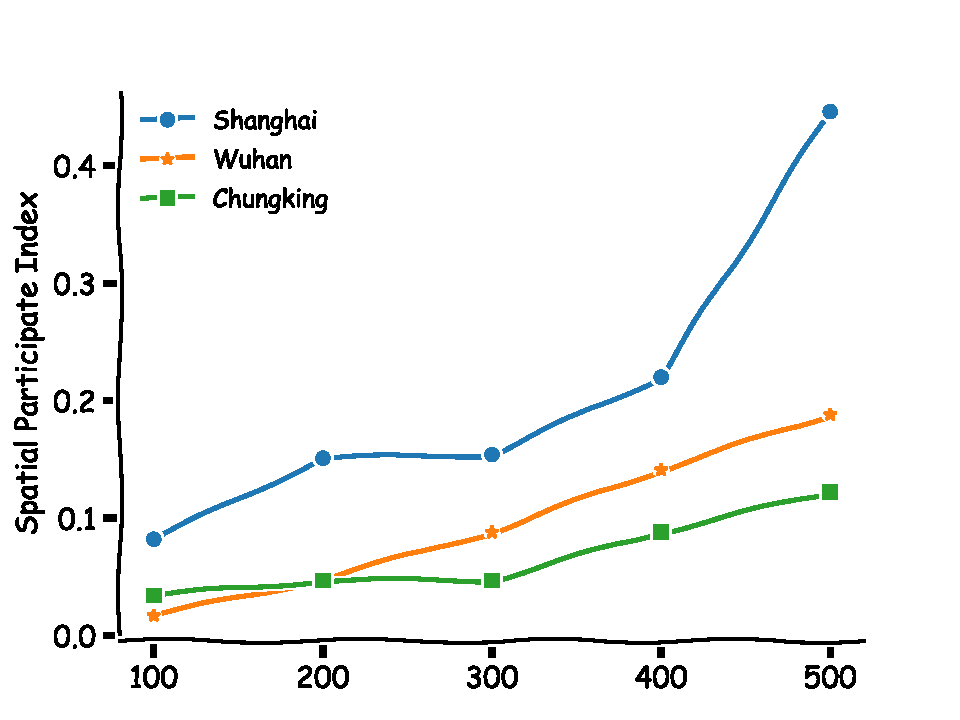
\includegraphics[scale=0.6]{figures/Participate.pdf}
\end{frame}

\begin{frame}[c]{POI空间分析(同位模式)}
    北京市POI空间模式,$d=500$m,空间参与度阈值为$0.6$

    \begin{itemize}
        \footnotesize
        \pause
        \item \textbf{二阶(29)}

        (中餐厅,校园生活),(校园生活,医院),(甜品店,中餐厅),(咖啡厅,校园生活),(咖啡厅,酒吧),(清真餐馆,酒吧) $\ldots$

        \pause
        \item \textbf{三阶(29)}

        (中餐厅,校园生活,医院),(电影院,KTV,美容美发店),
        (甜品店,中餐厅,美容美发店),(美容美发店,酒吧,甜品店),(中餐厅,校园生活,咖啡厅) $\ldots$

        \pause
        \item \textbf{四阶(19)}

        (电影院,KTV,咖啡厅,美容美发店),(KTV,中餐厅,甜品店,美容美发店),
        (甜品店,中餐厅,咖啡厅,美容美发店),(甜品店,咖啡厅,美容美发店,酒吧)$\ldots$

        \pause
        \item \textbf{五阶(7)}

        电影院,KTV,咖啡厅,甜品店,美容美发店),(KTV,中餐厅,咖啡厅,美容美发店,酒吧),
        (甜品店,中餐厅,咖啡厅,美容美发店,酒吧)$\ldots$

        \pause
        \item \textbf{六阶(1)}

        (KTV,中餐厅,咖啡厅,甜品店,美容美发店,酒吧)
    \end{itemize}
\end{frame}